\documentclass{beamer}

\usepackage{Haust2016glærur}

\title{Tölvunarfræði 1a}
\subtitle{Vika 1, seinni fyrirlestur}

\begin{document}

\begin{frame}
\titlepage
\end{frame}

\section{Inngangur}

\begin{frame}{Í síðasta þætti\ldots}
\begin{itemize}
 \item Kynning á námskeiðinu
 \item Forritunarhugtakið
 \item Hvað Matlab er
 \begin{itemize}
  \item Hvernig gekk að setja það upp?
 \end{itemize}
 \item Bitar og tvíundartölur
 \item Breytur
\end{itemize}
\end{frame}

\begin{frame}{Bók}
Bókin ku vera til í mismunandi útgáfum
\begin{columns}
\column{0.5\textwidth}
\begin{center}
3. útgáfa

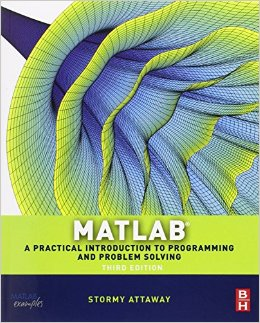
\includegraphics[width=0.66\linewidth]{../Pics/matlab_stormy}
\end{center}
\column{0.5\textwidth}
\begin{center}
4. útgáfa


\includegraphics[width=0.7\linewidth]{../Pics/matlab_stormy_v4}
\end{center}
\end{columns}
Munum gera ráð fyrir að báðar útgáfur séu í notkun
\end{frame}

\begin{frame}{Piazza!}
\label{frame:piazza}
\begin{itemize}
 \item Spjallkerfið \href{piazza.com/hi.is/fall2016/tl105g}{Piazza} verður notað í þessu námskeiði
 \begin{itemize}
  \item \url{piazza.com/hi.is/fall2016/tl105g}
 \end{itemize}
 \item Kerfið mun vera besta leiðin til að fá svör frá samnemendum, dæmatímakennurum og undirrituðum
 \item Piazza eða tölvupóstur?
 \begin{itemize}
  \item Málið getur átt við fleiri $\to$ Piazza
  \begin{itemize}
   \item Spurningar um heimadæmi
   \item Spurningar um tímasetningar
   \item Spurningar um námskeiðið
  \end{itemize}
  \item Málið er persónulegt $\to$ tölvupóstur
 \end{itemize}
\end{itemize}
\end{frame}

\begin{frame}{Matlab-skipanaglugginn}
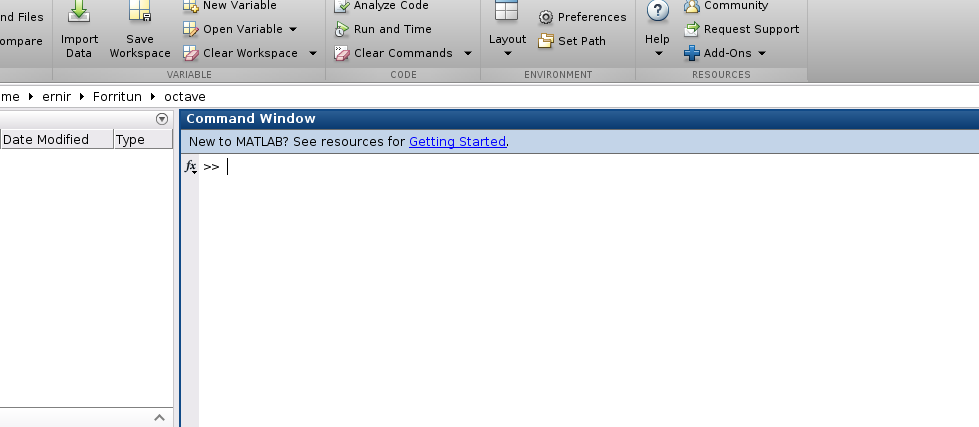
\includegraphics[width=\textwidth]{../Pics/command-window}
\end{frame}

\begin{frame}{Matlab-skipanaglugginn}
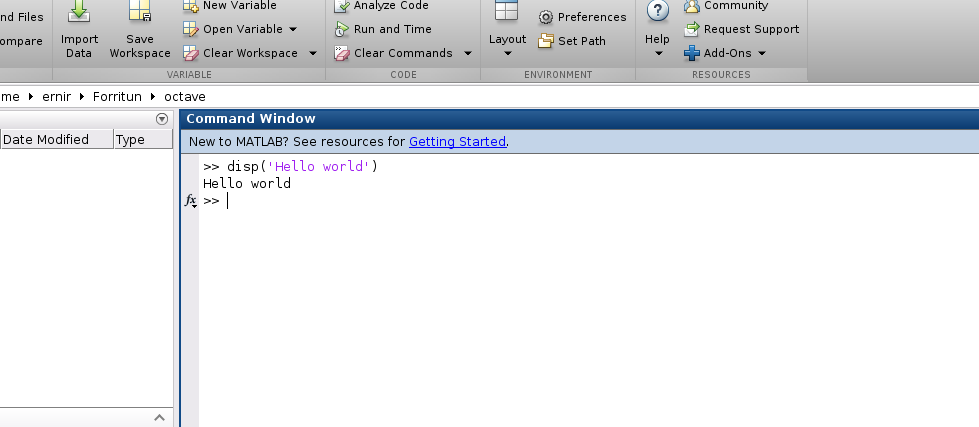
\includegraphics[width=\textwidth]{../Pics/command-window-hello-world}
\end{frame}

\section{Útreikningar}

\begin{frame}[fragile]{Reiknisegðir}
\begin{columns}
\column{0.5\textwidth}
\begin{itemize}
 \item Við getum reiknað með Matlab á mjög svipaðan hátt og í (mjög öflugri) reiknivél
 \begin{itemize}
  \item \texttt{+}, \texttt{-}: samlagning og frádráttur
  \item \texttt{*}, \texttt{/}, \texttt{\textbackslash}: margföldun, deiling, deilt uppí
  \item \texttt{\^}: veldishafning
 \end{itemize}
 \item Munum að við getum notað breytur!
\end{itemize}
\column{0.5\textwidth}
\begin{minted}[frame=lines]{matlab}
>> height = 4;
>> width = 2.5;
>> area = height * width
area =  10
\end{minted}
\end{columns}
\end{frame}

\begin{frame}{Forgangur}
Líkt og í hefðbundinni stærðfræði, þá eru sumir virkjar (e. \emph{operators}) framkvæmdir á undan öðrum.
\begin{center}
\begin{tabular}{ll}
\toprule
Virki&Hópur\\
\midrule
\texttt{()}&Svigar\\
\texttt{\^}&Veldishafning\\
\texttt{-}&Viðsnúningur formerkis\\
\texttt{*, /, \textbackslash}&Margföldun og deiling\\
\texttt{+, -}&Samlagning og frádráttur\\
\bottomrule
\end{tabular}
\end{center}
Virkjar efst í töflunni eru framkvæmdir fyrst.
\end{frame}

\begin{frame}[fragile]{Forgangur aðgerða}
\begin{itemize}
 \item Matlab les frá vinstri til hægri ef um ``jafntefli'' er að ræða
\begin{minted}[frame=lines]{matlab}
>> 1/2*2
ans =
     1
\end{minted}
 \item Notið sviga ef þið eruð í vafa
\end{itemize}
\end{frame}

\section{Föll}

\begin{frame}[fragile]{Föll í Matlab}
\begin{itemize}
 \item Föll eru lykilfyrirbrigði í forritun.
 \item Matlab er með innbyggð föll sem hægt er að nota:
\end{itemize}
\begin{minted}[frame=lines]{matlab}
>> sin(pi/2)
ans =  1
>> cos(0)
ans =  1
\end{minted}
\end{frame}

\begin{frame}{Innbyggð föll}
\begin{itemize}
 \item Mjög mikið er til af innbyggðum stærðfræðiföllum
 \item \texttt{sin, cos, tan, asin, acos, atan, exp, log, log10, sqrt, abs, round, mod, rem,}\ldots
 \item Nokkur föll breyta kommutölum í heiltölur:
 \begin{itemize}
  \item \texttt{floor(x)}: rúnnar niður að $-\infty$
  \item \texttt{ceil(x)}: rúnnar upp að $+\infty$
  \item \texttt{fix(x)}: rúnnar að núlli
  \item \texttt{round(x)}: rúnnar að næstu heiltölu
 \end{itemize}
 \item \texttt{>> help elfun} gefur lista
\end{itemize}
\end{frame}

\begin{frame}[fragile]{Frekari upplýsingar}
Til að fá snöggt yfirlit yfirlit yfir innbyggt fall má skrifa \texttt{help} og svo nafn fallsins:
\begin{minted}[frame=lines]{matlab}
>> help sin
\end{minted}
eða \texttt{doc} og svo nafn fallsins til að skoða það í hjálpinni:
\begin{minted}[frame=lines]{matlab}
>> doc sin
\end{minted}
Hjálpin í Matlab er almennt mjög gagnleg.
\end{frame}

\begin{frame}[fragile, shrink]{Dæmi um útreikninga}
\vspace{1cm}
Lausn á annars stigs jöfnunni $x^2 + 3x - 4 = 0$
\begin{minted}[frame=lines]{matlab}
>> a = 1;
>> b = 3;
>> c = -4;
>> x1 = (-b + sqrt(b^2 - 4*a*c))/(2*a)
x1 =
      1
>> x2 = (-b - sqrt(b^2 - 4*a*c))/(2*a)
x2 =
     -4
\end{minted}
\end{frame}

\begin{frame}[fragile]{Deilingarafgangar}
\begin{itemize}
 \item Hugmyndin um ``deilingarafgang'' kemur furðu oft fyrir í tölvunarfræði
 \item Dæmi um deilingarafgang: Þegar 10 er deilt með 3 gengur einn af. Þetta er táknað með lykilorðinu \emph{mod}:
 \begin{itemize}
  \item $10 \Mod{3} = 1$
 \end{itemize}
 \item Í Matlab má nota fallið \texttt{mod}:
\end{itemize}
\begin{minted}[frame=lines]{matlab}
>> mod(10,3)
ans =
     1
\end{minted}
\begin{itemize}
 \item Einnig er til fallið \texttt{rem}, sem er svipað en höndlar neikvæðar tölur á annan hátt
\end{itemize}
\end{frame}

\section{Slembitölur}

\begin{frame}{Hvað eru slembitölur?}
\begin{itemize}
 \item Slembitölur (e. \emph{random numbers}) eru tölur búnar til ``af handahófi''
 \item Ein stök tala er ekki slembin
 \item Getum skoðað runu af tölum og leitt líkur að því að hún sé slembin
\end{itemize}
\end{frame}

\begin{frame}[fragile]{Slembitölur í Matlab}
\begin{itemize}
 \item Fallið \texttt{rand} býr til jafndreifðar slembitölur
 \item Býr til kommutölur frá 0 til 1 (hvorug meðtalin!)
\end{itemize}
\begin{minted}[frame=lines]{matlab}
>> r1 = rand()
r1 =
    0.8147
>> r2 = rand()
r2 =
    0.9058
\end{minted}
\end{frame}

\begin{frame}{Slembitölugjafar}
\begin{itemize}
 \item Erfitt er að búa til ``raunverulegan'' slembitölugjafa (e. \emph{random number generator})
 \item Við notum reiknirit (e. \emph{algorithms}) til að búa til slembitölur
 \begin{itemize}
  \item Oft kallaðar gervislembitölur (e. \emph{pseudo-random numbers})
  \item Reikniritin geta engu að síður orðið ansi góð \pause
  \item \ldots og ansi léleg
 \end{itemize}
\end{itemize}
\end{frame}

\begin{frame}{Slembitölugjafar í tölvum}
\begin{columns}
\column{0.6\textwidth}
Notum stærðfræðiformúlu:
\[
r_{n+1} = (ar_n + c) \Mod{m}
\]
veljum okkur $a=3$, $c=4$, $m=10$, setjum $r_0 = 0$ og reiknum:
\begin{align*}
r1 = (3 \cdot 0 + 4) \Mod{10}  &=  4\\
r2 = (3 \cdot 4 + 4) \Mod{10}  &=  6\\
r3 = (3 \cdot 6 + 4) \Mod{10}  &=  2\\
r4 = (3 \cdot 2 + 4) \Mod{10}  &=  0\\
\end{align*}
\column{0.4\textwidth}
\begin{itemize}
\item Nú erum við komin í hring, fáum alltaf sömu niðurstöður
 \begin{itemize}
  \item Góðir slembitölugjafar eru með mun lengri hring
 \end{itemize}
 \item Þessi aðferð kallast línuleg samleifaraðferð (e. \emph{linear congruential method}). Formúla af þessari gerð kallast rakningarvensl (e. \emph{recurrence relation})
\end{itemize}
\end{columns}
\end{frame}

\begin{frame}{Upphafsgildi slembitölugjafa}
\begin{itemize}
 \item Matlab alltaf sama upphafsgildið í upphafi, svo 0.8147 er alltaf fyrsta slembitalan eftir ræsingu
 \begin{itemize}
  \item Hægt að breyta því með fallinu \texttt{rng}
 \end{itemize}
 \item Hægt að setja upphafsgildið á marga vegu:
 \begin{itemize}
  \item \texttt{rng('shuffle')}:upphafsstillt með kerfisklukkunni
  \item \texttt{rng('default')}: upphaflegt upphafsgildi
  \item \texttt{rng(tala)}: upphafsstillt með gildinu \texttt{tala}
 \end{itemize}
\end{itemize}
\end{frame}

\begin{frame}[shrink]{Upphafsgildið}
\vspace{1cm}
\begin{itemize}
 \item Slembitölugjafi samanstendur af mjög löngum hring af slembitölum
 \begin{itemize}
  \item Upphafsgildið ræður því hvar í hringnum við byrjum
  \item \texttt{rand} skilar svo næstu tölu á hringnum
 \end{itemize}
\end{itemize}
\begin{center}
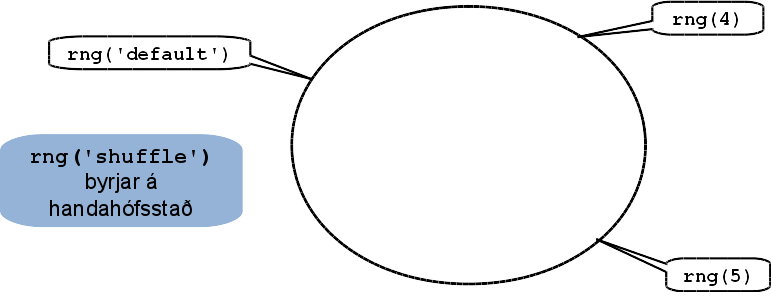
\includegraphics[width=0.7\textwidth]{../Pics/random-circle}
\end{center}
\end{frame}

\begin{frame}[fragile]{Dæmi um slembitölur}
\vspace{-0.5cm}
\begin{columns}
\column{0.6\textwidth}
\begin{minted}[frame=lines]{matlab}
>> r = rand()*10
r =
    9.0579
\end{minted}
\column{0.4\textwidth}
Kommutala á bilinu $]0;10[$
\end{columns}

\begin{columns}
\column{0.6\textwidth}
\begin{minted}[frame=lines]{matlab}
>> low = 5;
>> high = 12;
>> r = rand()*(high-low)+low
r =  7.7613
\end{minted}
\column{0.4\textwidth}
Kommutala á bilinu $]5;12[$
\end{columns}
\end{frame}

\begin{frame}[fragile]{Slembnar heiltölur}
\texttt{rand} fallið býr til slembnar kommutölur - til að gera slembnar heiltölur þarf önnur föll (eða smá fimleika)
\begin{columns}
\column{0.6\textwidth}
\begin{minted}[frame=lines]{matlab}
>> randomInteger = randi(20)
randomInteger =  8
\end{minted}
\column{0.4\textwidth}
Heiltölur á bilinu $[1;20]$
\end{columns}

\begin{columns}
\column{0.6\textwidth}
\begin{minted}[frame=lines]{matlab}
>> randomInteger = randi([4, 8])
randomInteger =  6
\end{minted}
\column{0.4\textwidth}
Heiltala á bilinu $[4; 8]$. (Hornklofarnir í Matlab-kóðanum skýrast seinna)
\end{columns}
\end{frame}

\begin{frame}{Fyrirlestraræfing}
Skráið ykkur inn á \url{http://socrative.com/} og gerið fyrstu fjórar spurningarnar.

Herbergisnúmer = \texttt{TOL105G2016}

Notendanafn = HÍ-tölvupóstfang
\end{frame}

\section{Bókstafir}

\begin{frame}[fragile]{Bókstafir}
\begin{itemize}
 \item Hægt er að vinna með bókstafi og (önnur tákn) í Matlab.
 \item Notum einfaldar gæsalappir til að tákna þá
 \begin{itemize}
  \item T.d. \texttt{'a'}, \texttt{'E'}, \texttt{'\%'} og \texttt{'4'}
 \end{itemize}
 \item Athugum að það er munur á stafnum \texttt{'4'} (kóðaður \texttt{0110100} í ASCII) og tölunni $4$ (kóðuð \texttt{00000100}).
\end{itemize}
\begin{minted}[frame=lines]{matlab}
>> myChar = 'E'
myChar =
E
\end{minted}
\end{frame}

\begin{frame}{Að geyma bókstafi í tölvu}
\begin{columns}
\column{0.6\textwidth}
\begin{itemize}
 \item Möguleg leið til að kóða bókstafi og önnur tákn er ASCII
 \item Einföld kóðunaraðferð, mjög gömul
 \begin{itemize}
  \item Tákn gefin með 7 bitum
  \begin{itemize}
   \item ``Efsti'' bitinn notaður sem varbiti (e. \emph{parity bit})
  \end{itemize}
 \end{itemize}
 \item Líklega mest notaða kóðunaraðferðin í dag: UTF-8
 \begin{itemize}
  \item ASCII er innifalið í UTF-8
 \end{itemize}
\end{itemize}
\column{0.4\textwidth}
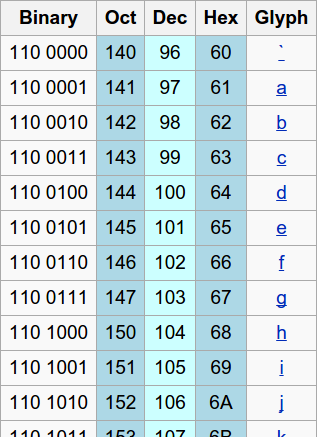
\includegraphics[width=\linewidth]{../Pics/ascii-table}
\\Hluti ASCII-töflunnar af \href{https://en.wikipedia.org/wiki/ASCII}{Wikipedia}
\end{columns}
\end{frame}

\begin{frame}[fragile]{Föll fyrir kóðun}
\begin{itemize}
 \item Við getum fundið kóðann fyrir einstaka bókstafi
 \item Dæmi: Stafurinn \texttt{'Þ'} sem 32 bita heiltala: 
\begin{minted}[frame=lines]{matlab}
>> int32('Þ')
ans =
         222
\end{minted}
 \item Einnig er hægt að fara í hina áttina:
\begin{minted}[frame=lines]{matlab}
>> char(222)
ans =
Þ
\end{minted}
\end{itemize}
\end{frame}

\section{Rökyrðingar}

\begin{frame}{Rökyrðingar}
\begin{itemize}
 \item Rökyrðingar (e. \emph{logical expressions}) vinna með \emph{sanngildi} í stað talna.
 \begin{itemize}
  \item Sanngildi eru tvö: \texttt{true} og ósatt \texttt{false}
  \item Í Matlab er oft notað $1$ og $0$ í stað \texttt{true} og \texttt{false}
 \end{itemize}
 \item Notum nýja virkja (e. \emph{operators}). Tvær gerðir:
 \begin{itemize}
  \item Samanburðarvirkjar (\emph{relational})
  \item Rökvirkjar (\emph{logical})
 \end{itemize}
\end{itemize}
\end{frame}

\subsection{Samanburðarvirkjar}
\begin{frame}{Samanburðarvirkjar}
\begin{columns}
\column{0.5\textwidth}
\begin{itemize}
 \item Samanburðarvirkjar bera saman gildi og skila sanngildi (e. \emph{truth value}).
 \item Sanngildi hafa sitt eigið tag, \texttt{logical}\footnotemark
\end{itemize}
\column{0.5\textwidth}

\vspace{0.5cm}
Samanburðarvirkjar í Matlab: 

\vspace{0.2cm}
\begin{tabular}{ll}
\toprule
Virki&Merking\\
\midrule
\texttt{>}&stærri en\\
\texttt{<}&minni en\\
\texttt{>=}&stærri en eða jafn ($\geq$)\\
\texttt{<=}&minni en eða jafn ($\leq$)\\
\texttt{==}&jafnt og\\
\texttt{\~}\texttt{=}&ekki jafnt og\\
\bottomrule
\end{tabular}
\end{columns}
\footnotetext{Við höfum núna líka séð \texttt{double}, \texttt{char} og \texttt{int32}.}
\end{frame}

\begin{frame}[fragile]{Sanngildi}
Í Matlab er sanngildið ``satt'' oftast táknað með \texttt{logical} gildinu \texttt{1} og ``ósatt'' með \texttt{logical} gildinu \texttt{0}.
\begin{columns}
\column{0.5\textwidth}
\begin{minted}[frame=lines]{matlab}
>> 2 < 3
ans =
     1
\end{minted}
\begin{minted}[frame=lines]{matlab}
>> 3 >= 2
ans =
     1
\end{minted}
\column{0.5\textwidth}
\begin{minted}[frame=lines]{matlab}
>> 'b' < 'a'
ans =
     0
\end{minted}

\vspace{0.09cm}
Öll svörin eru af taginu \texttt{logical}, þó þau líti út eins og venjulegar tölur (sem væru af tagi eins og \texttt{double} eða \texttt{int32}).
\end{columns}
\end{frame}

\subsection{Rökvirkjar}
\begin{frame}{Rökvirkjar}
Rökvirkjar vinna með sanngildi:
\begin{center}
\begin{tabular}{ll}
\toprule
Virki&Merking\\
\midrule
||& eða\footnotemark, skilar satt ef annað viðfangið er satt\\
\&\& & og\footnotemark[1], skilar satt ef bæði viðföngin eru sönn\\
\~{} &ekki, skilar öfugu við viðfangið\\
\bottomrule
\end{tabular}
\end{center}
Einnig er til rökfallið \texttt{xor}. Það tekur tvö viðföng og skilar ``annaðhvort eða''. Satt ef annað viðfangið er satt, en ekki ef bæði eru sönn.
\footnotetext{Þessir virkjar eiga við stök sanngildi. Virkjar fyrir vigra koma seinna.}
\end{frame}

\begin{frame}[fragile]{Dæmi um rökvirkja}
\begin{columns}
\column{0.5\textwidth}
\begin{minted}[frame=lines]{matlab}
>> (2 < 4) || (2 > 4)
ans =
     1
\end{minted}
\begin{minted}[frame=lines]{matlab}
>> (2 < 4) && (2 > 4)
ans =
     0
\end{minted}
\column{0.5\textwidth}
\begin{minted}[frame=lines]{matlab}
>> ~(2 < 4)
ans =
     0
\end{minted}
\begin{minted}[frame=lines]{matlab}
>> xor(2 < 4, 2 > 4)
ans =
     1
\end{minted}
\end{columns}
\end{frame}

\begin{frame}{Sanntöflur rökvirkja}
\begin{columns}
\column{0.33\textwidth}
\begin{center}
Eða\\
\begin{tabular}{ccc}
\toprule
\texttt{x}&\texttt{y}&\texttt{x||y}\\
\midrule
1&1&1\\
1&0&1\\
0&1&1\\
0&0&0\\
\bottomrule
\end{tabular}
\end{center}
\column{0.33\textwidth}
\begin{center}
Og\\
\begin{tabular}{ccc}
\toprule
\texttt{x}&\texttt{y}&\texttt{x\&\&y}\\
\midrule
1&1&1\\
1&0&0\\
0&1&0\\
0&0&0\\
\bottomrule
\end{tabular}
\end{center}
\column{0.33\textwidth}
\begin{center}
XOR\\
\begin{tabular}{ccc}
\toprule
\texttt{x}&\texttt{y}&\texttt{xor(x,y)}\\
\midrule
1&1&0\\
1&0&1\\
0&1&1\\
0&0&0\\
\bottomrule
\end{tabular}
\end{center}
\end{columns}
\end{frame}

\begin{frame}{Forgangur virkja}
\vspace{-0.5cm}
Stækkum forgangstöfluna:
\begin{center}
\small
\begin{tabular}{ll}
\toprule
Virki&Hópur\\
\midrule
\texttt{()}&Svigar\\
\texttt{'} og \texttt{\^}&Bylt og veldi\\
\texttt{-} og \texttt{\~{}}&Viðsnúningur formerkis og neitun\\
\texttt{*, /, \textbackslash}&Margföldun og deiling\\
\texttt{+, -}&Samlagning og frádráttur\\
\texttt{:}&Tvípunktur (fyrir vigra)\\
\texttt{<}, \texttt{<=}, \texttt{>}, \texttt{>=}, \texttt{==}, \texttt{\~{}=}&Samanburður\\
\texttt{\&\&}&Og\\
\texttt{||}&Eða\\
\texttt{=}&Gildisveiting\\
\bottomrule
\end{tabular}
\end{center}
Virkjar efst í töflunni eru framkvæmdir fyrst.
\end{frame}

\begin{frame}{Fyrirlestraræfing}
Skráið ykkur inn á \url{http://socrative.com/} og klárið fyrirlestraræfinguna.

Herbergisnúmer = \texttt{TOL105G2016}

Notendanafn = HÍ-tölvupóstfang
\end{frame}



\end{document}
